\documentclass{article}
\usepackage{graphicx}
\usepackage{mathtools}
\usepackage{xfrac}
\usepackage{amsmath, amssymb}
\usepackage{listings}
\usepackage{float}
\usepackage{wrapfig}
\usepackage{tikz}
\usepackage{fullpage}
\usepackage{hyperref}
\usepackage{mathalpha}
\usepackage{tikz}
\usepackage{cite}
\usepackage{amsthm}

\newtheorem{theorem}{Proposition}[section]
\newtheorem{corollary}{Corollary}[theorem]
\newtheorem{lemma}[theorem]{Lemma}

\theoremstyle{definition}
\newtheorem{definition}{Definition}[section]

\theoremstyle{remark}
\newtheorem*{remark}{Remark}
\newtheorem*{example}{Example}
\newtheorem*{notation}{Notation}

\title{Computer Simulation Assignment 1}
\author{David Lawton\\ Student No.: 22337087}
\date{28th Sep. 2024.}

\begin{document}

\maketitle

\tableofcontents


\section{Introduction}
This report is a summary of the work done for the first assignment of the Computer Simulation 1 module, the first part examines the Heron's root finding method and the second part answers quastions from sections 1.3 and 1.4 from Landau and Paez's "Computational Problems for Physics". The assignment was written in Python using classes and methods to allow seperate parts to be run easily, and to prevent any variables in seperate sections from being unintentionally reused. The code is attached in the file "CompSimAssignment1\_DavidLawton.py".

\section{Heron's Root Finding Method}

Heron's method is a root finding algorithm that uses the iterative formula:

\begin{equation}
    x_{n+1} = \frac{1}{2} \left( x_n + \frac{a}{x_n} \right)
\end{equation}
where $x_0$ is the initial guess and a is the number we are trying to find the square root of. As $n\rightarrow\infty$, $x_n$ converges to $\sqrt{a}$. The first step of coding this method was to code the iterative formula in Python:
\begin{lstlisting}{language=Python}
    def HeronRFM(self, x_n, a):
        x = 0.5 * (x_n + a / x_n)
        return x
\end{lstlisting}

We then used this module to find the square root of 2, for a couple of initial guesses $\left\{ 1, 2 \right\} $, and printed the results. We also plotted these results on a graph to show the convergence of the method, the error of $x_n^2$, and the convergence of $x_n^2$ to $2$:\\
\hspace{-4cm}
\begin{figure}[H]
    \centering
    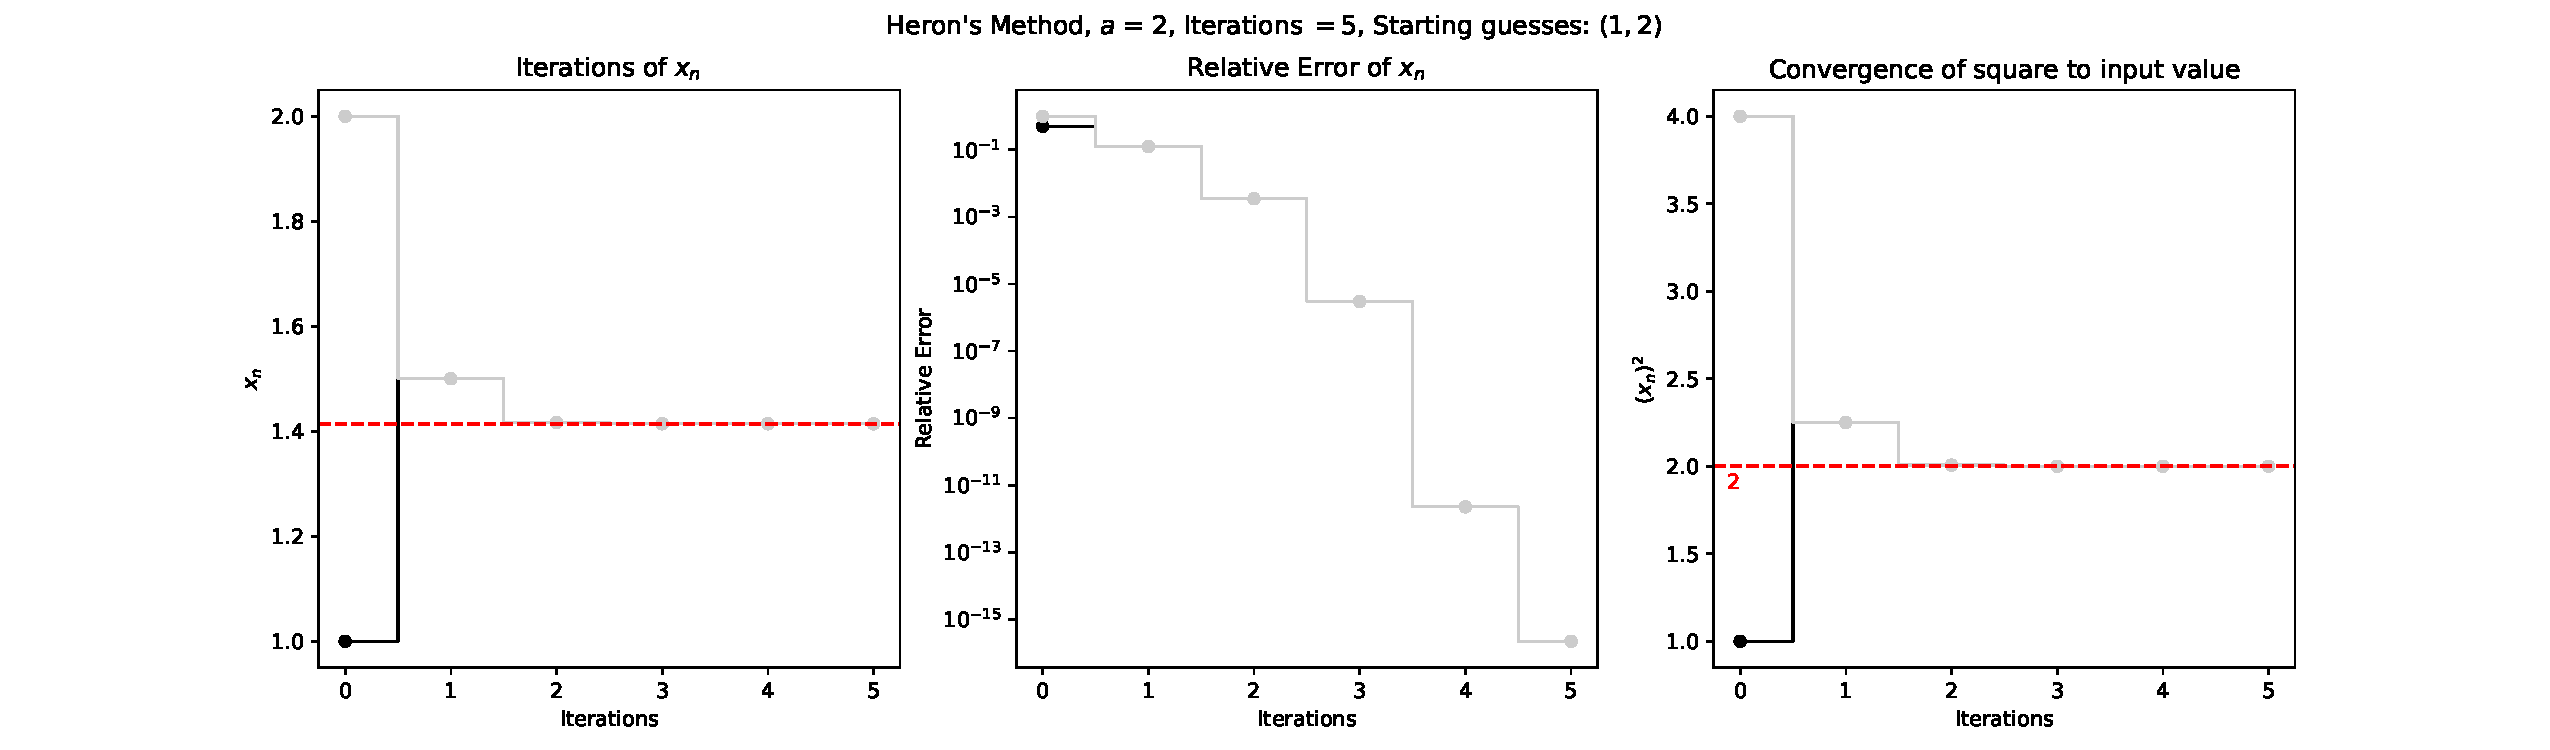
\includegraphics[width=1.2\textwidth]{HeronRMF2.pdf}
    \caption{\label{fig:HeronRMF2} Plot of Heron's Root finding method for $a = 2$. (a) shows the convergence of $x_n$ to $x_5$ which we show to be $\sqrt{2}$ in (b) and (c), (b) shows the relative error of $x_n^2$ from $2$, and (c) shows the convergence of $x_n^2$ to $2$.}
\end{figure}
As is clearly visible in figure \ref{fig:HeronRMF2}, the method converges to$x_5$, it is printed by the code that $x_5 = 1.414213562373095$. $(x_5)^2 = 1.9999999999999996$, with relative error of ~$10^{-15}$.

\section{Numerical Accuracy: Landau and Paez, section 1.3 questions}

\subsection{1.3 Question 1}
Question 1 asks us to determine our computer's overflow and underflow limits. We can do this by finding the largest and smallest numbers that can be stored in a float. This is done by multiplying and dividing, respectively, a starting number by 2 until, in the first case "np.isinf($x_n$)" is true, and in the second case $x_n = 0$. The code for this is found in the class UnderOverFlow in the attached code file. The results are printed below:
\begin{lstlisting}{language=Python}
    The underflow occured after 1075 iterations
    The underflow value is 5e-324.
    The overflow occured after 1023 iterations
    The overflow value is 8.98846567431158e+307.
\end{lstlisting}
We can conclude that the underflow limit is of the magnitude $10^{-324}$ and the overflow limit is of the magnitude $10^{307}$.
\subsection{1.3 Question 2}
In question 2, of section 1.3, we are asked to determine the machine precision of our computer, $\varepsilon_m$, up to a factor of 2. This is the largest number that can be added to 1 and still be stored as 1. We can find this by starting at an initial guess, $q = 1$, and adding it to 1, we then half it and add it to 1, continuously until the output is 1. This code can be found in the class "Precision" in the attached code file. The result is printed below:
\begin{lstlisting}{language=Python}
    The real machine precision is 1.1102230246251565e-16.
    The complex machine precision is 1.1102230246251565e-16.
\end{lstlisting}
Here the "complex precision" is complex analogue of real precision, and is the largest number that can be added to a fully complex number and still be stored as that number. \\
\indent We can can conclude that for any float, real or complex, there is a margin of error of $2.220446049250313e-16$. For complex floats written $a+ib$, $a,b\in\mathbb{R}$, $i=\sqrt{-1}$, the margin of error is the neighborhood of radius of $2.220446049250313e-16$ around the number.
\begin{remark}
    The neighborhood of radius $r$ of a complex number $z$ is the set of all complex numbers $z_i$ such that  $|z_i-z\leq r$.
\end{remark}

\subsection{1.4 Question 1}
For question 1 of section 1.4, we are asked to use forward and central difference algoritms to differentiate the functions $f(t) = \cos(t)$ and $g(t) = e^t$ at $t = 0.1, 1, 100$. The forward difference estimate of a derivative is defined:
\begin{equation}
    f'(t) = \frac{f(t+h) - f(t)}{h} + \mathcal{O}(h)
\end{equation}
The central difference estimate of a derivative is defined:
\begin{equation}
    f'(t) \approx \frac{f(t+h) - f(t-h)}{2h} + \mathcal{O}(h^2)
\end{equation}
The code for this is found in the class "difference\_methods" in the attached code file. A representative subset of the result, for $h=0.00015625$ are printed below:
\begin{lstlisting}{language=Python}
    The forward difference estimate of f'(0.1) is -0.09991115094152292.
    Error = 0.19974456758835107
    The central difference estimate of f'(0.1) is -0.09983341624071329.
    Error = 0.19966683288754145
    The forward difference estimate of g'(0.1) is 1.1052572640508629.
    Error = 8.634597521517406e-05
    The central difference estimate of g'(0.1) is 1.105170922573251.
    Error = 4.497603178776899e-09
\end{lstlisting}
We also produced plots of the error of the forward and central difference estimates of the derivatives of $f(t)$ and $g(t)$ at $t=0.1, 1, 100$:
\begin{figure}[H]
    \centering
    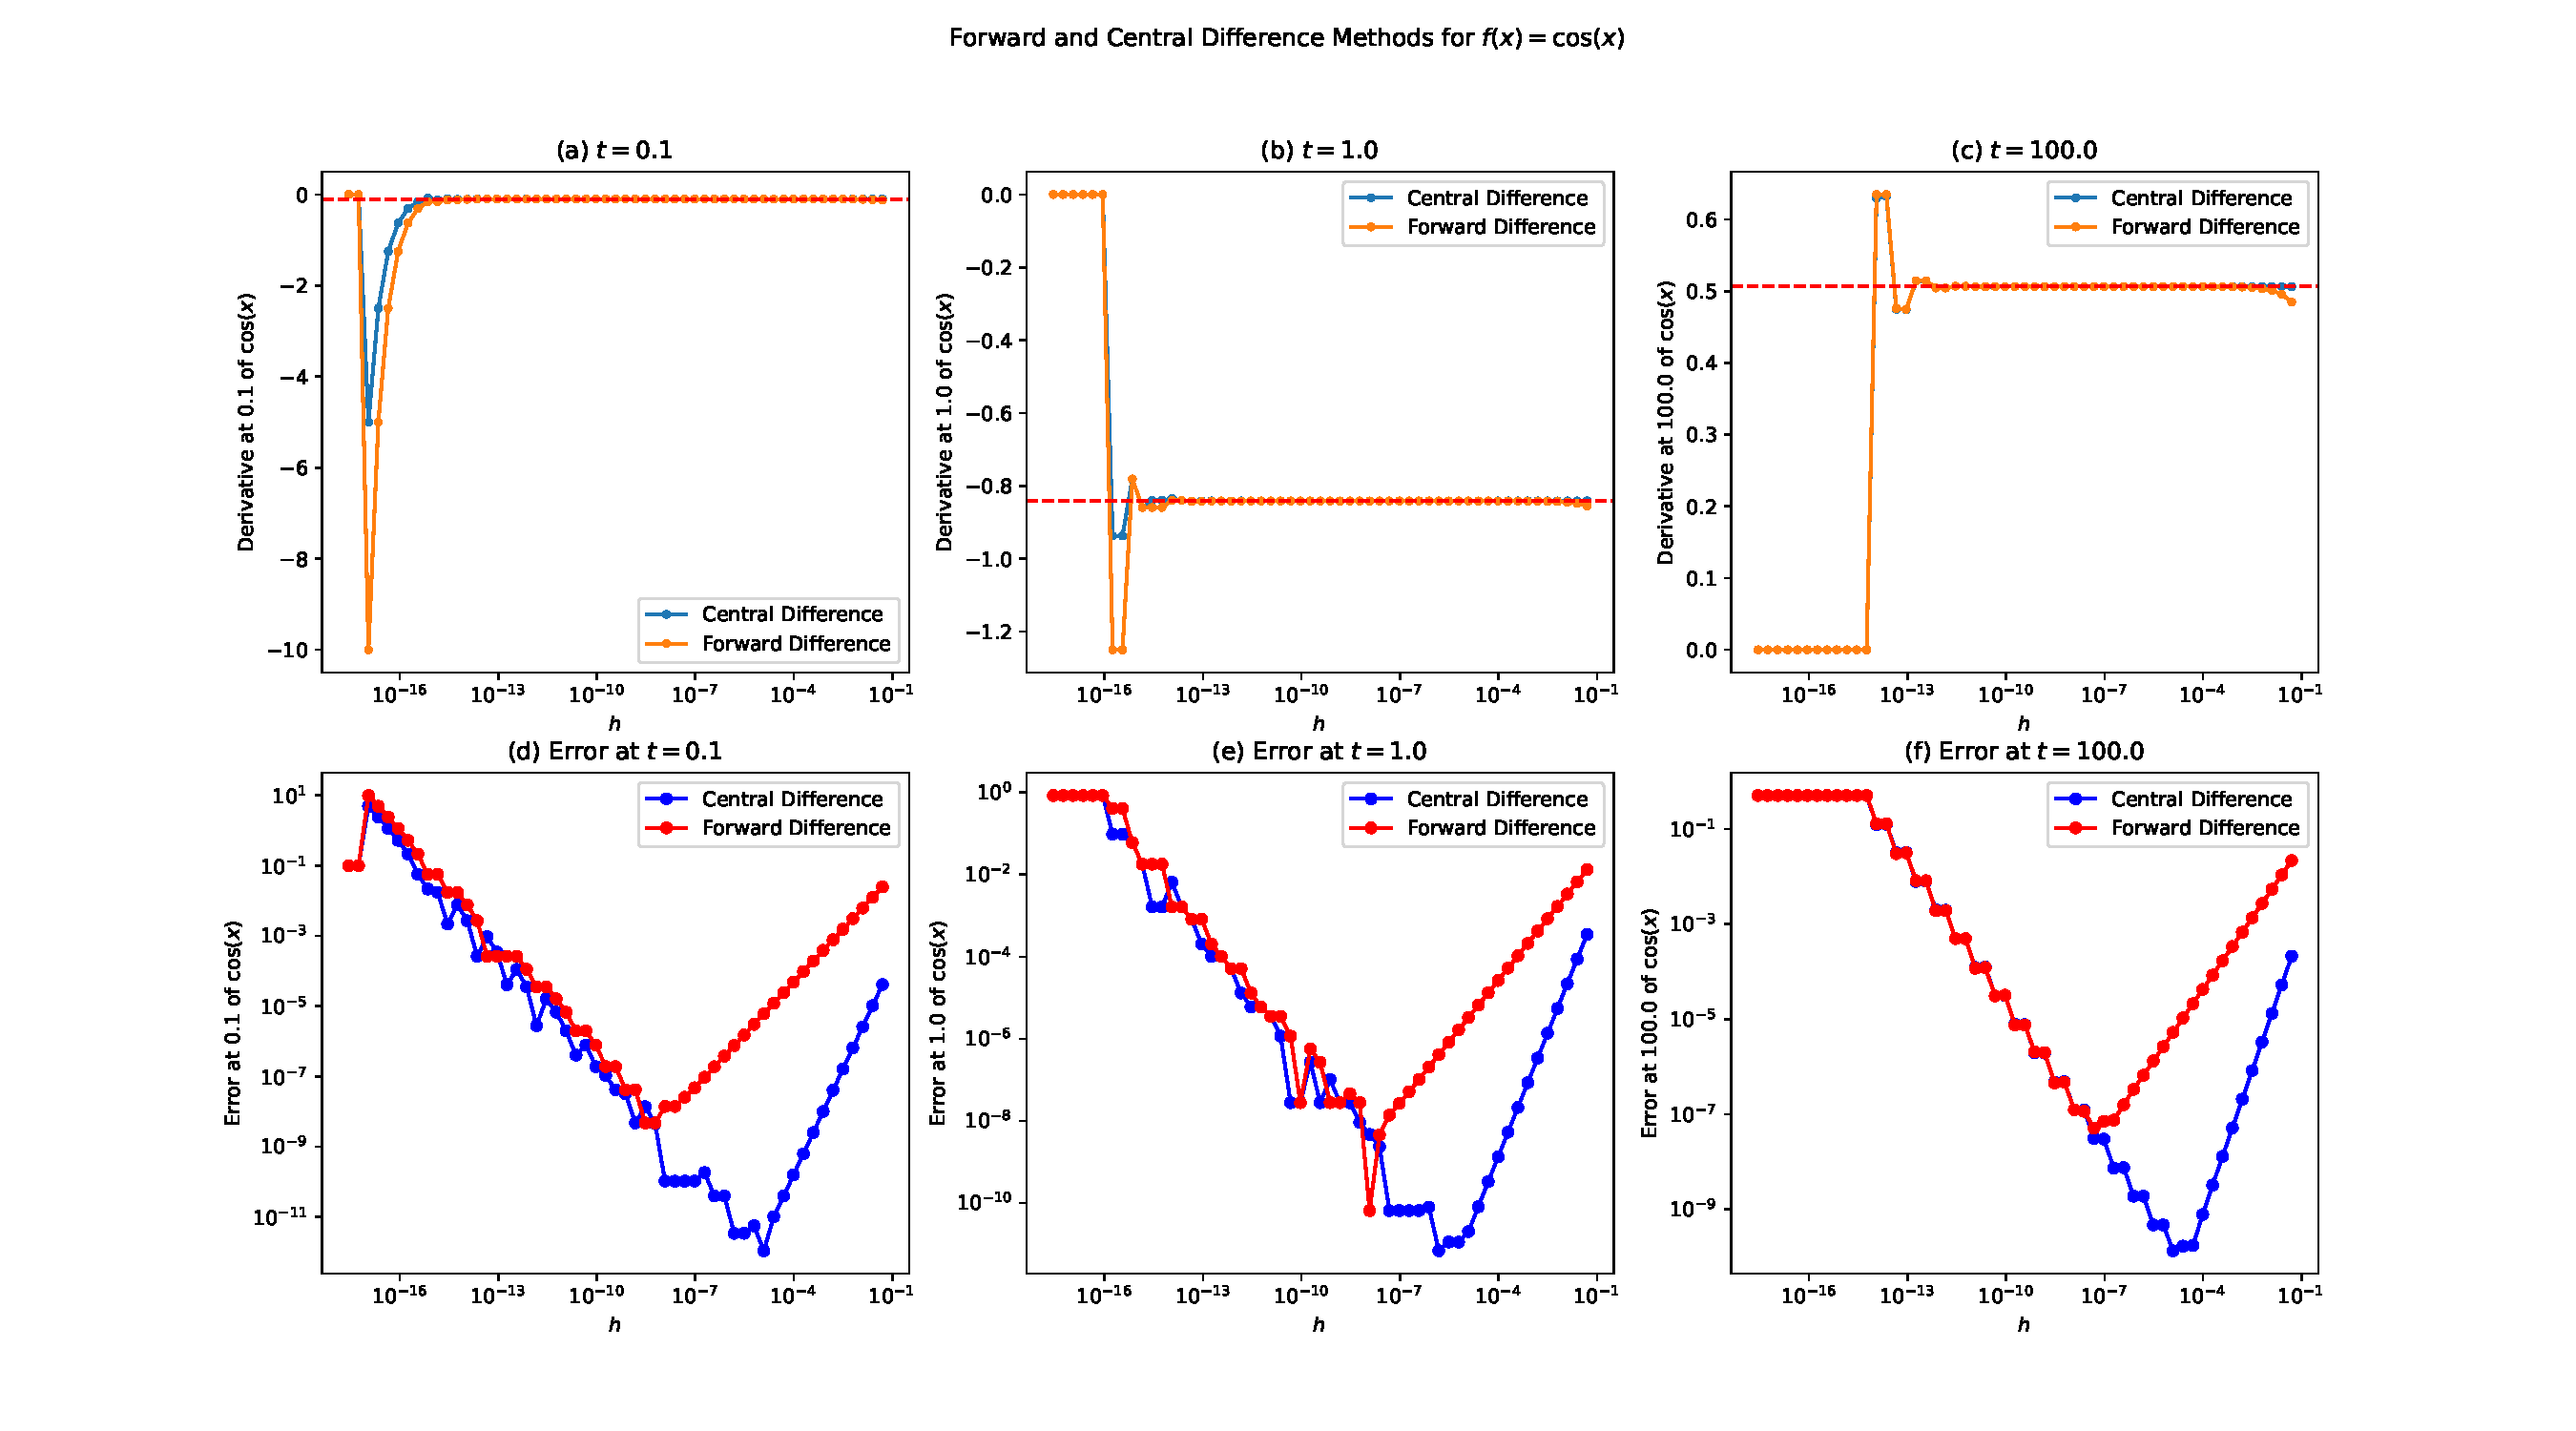
\includegraphics[width=1.2\textwidth]{DifferenceMethodsCos.pdf}
    \caption{\label{fig:DifferenceMethods} Plots for $f(t) = \cos(t)$, showing the value of the derivative and relative error, w.r.t. $h$, of the forward and central difference estimates of the derivative at $t=0.1, 1, 100$.\\
    \indent (a-c) show the value of the derivative of $f(t)$ at $t=0.1, 1, 100$, respectively. (d-f) show the relative error of the forward difference estimate of the derivative of $f(t)$ at $t=0.1, 1, 100$, respectively.}
\end{figure}

\begin{figure}[H]
    \centering
    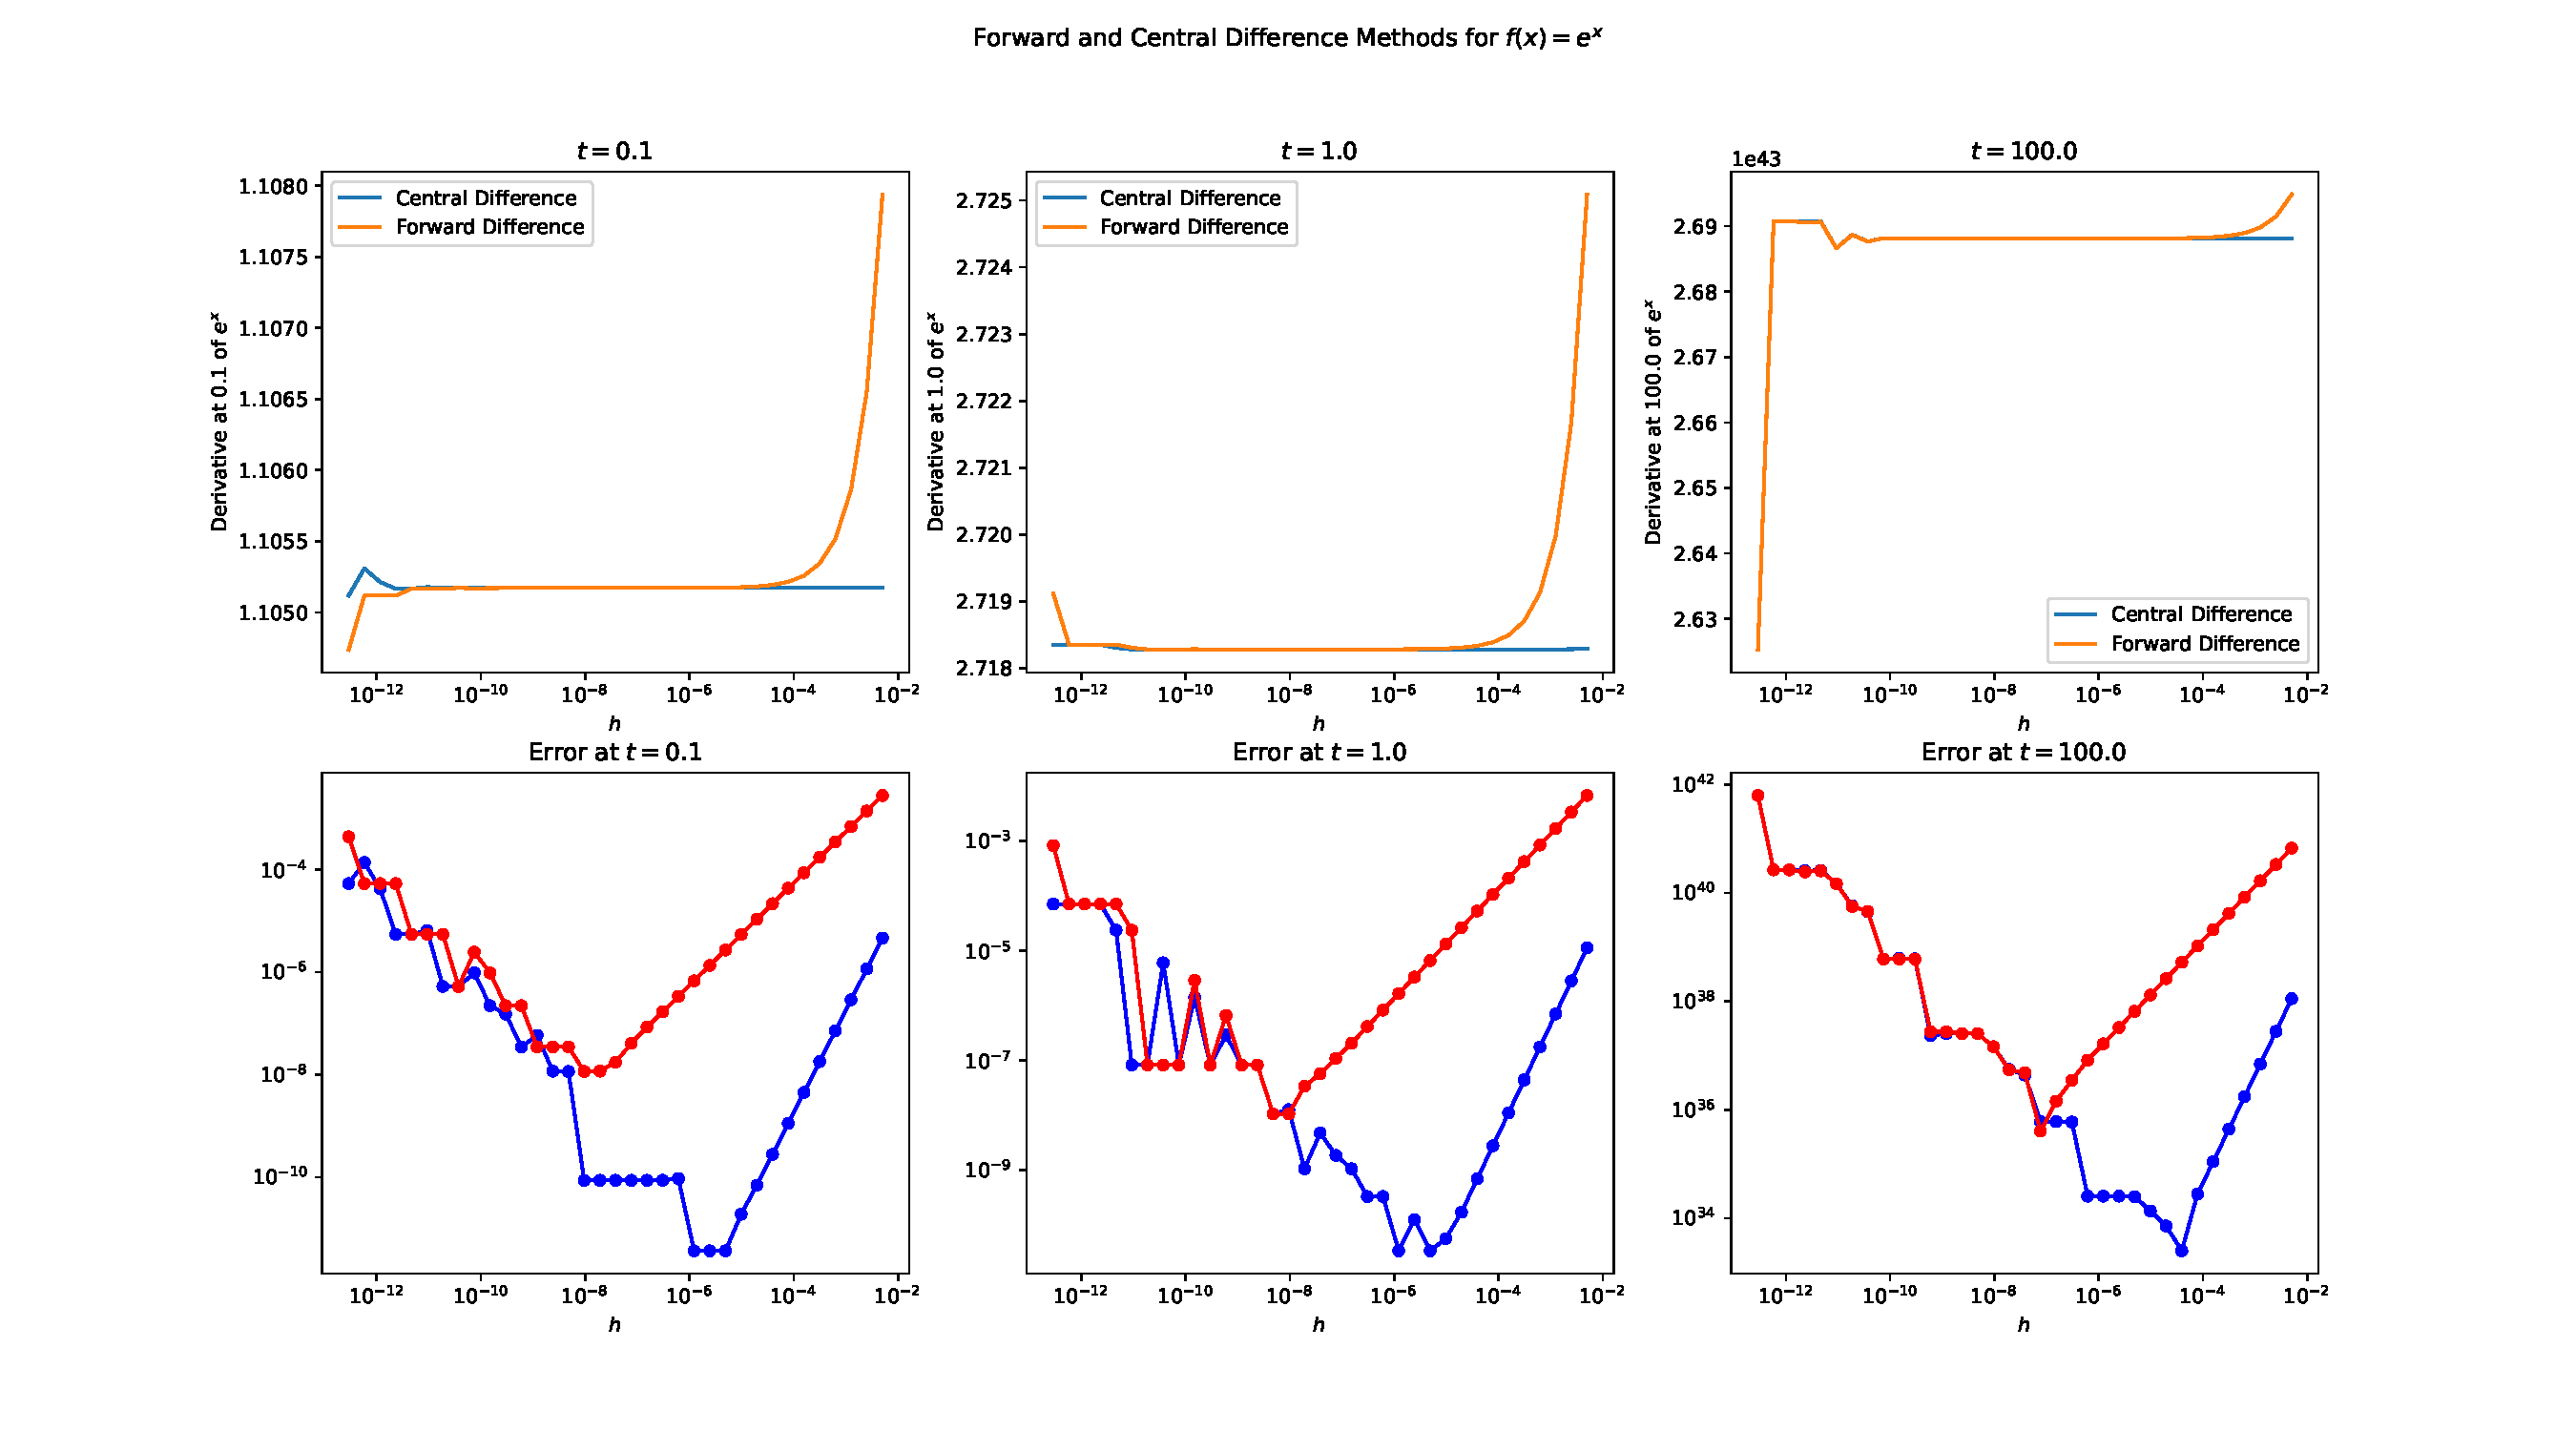
\includegraphics[width=1.2\textwidth]{DifferenceMethodsExp.pdf}
    \caption{\label{fig:DifferenceMethodsExp} Plots for $g(t) = e^t$, showing the value of the derivative and relative error, w.r.t. $h$, of the forward and central difference estimates of the derivative at $t=0.1, 1, 100$.\\
    \indent (a-c) show the value of the derivative of $g(t)$ at $t=0.1, 1, 100$, respectively. (d-f) show the relative error of the forward difference estimate of the derivative of $g(t)$ at $t=0.1, 1, 100$, respectively.}
\end{figure}
\indent As is visible in figures \ref{fig:DifferenceMethods} and \ref{fig:DifferenceMethodsExp}, the central difference estimate of the derivative is more accurate than the forward difference estimate, as the error of the central difference estimate is of order $h^2$, while the error of the forward difference estimate is of order $h$, as expected both become linear on the log-log plot, with slopes 2, 1 respectively. Interestingly, once the error reaches a line proportional to some negative power of $h$, the error diverges, this is due to the rounding error from the machine precision becoming more significant than the error of the difference estimate. Eventually when $h<\varepsilon_m\cdot t$, the relative error becomes 1, as $t+h$ is indistinguishable from $t$, and the derivative goes to 0.

\end{document}